%------ setup ------

\documentclass[11pt, a4paper]{article}

% set margins
\usepackage[a4paper, margin=2.5cm]{geometry}

% use Times New Roman
\usepackage{mathptmx}
\usepackage[T1]{fontenc}

% double line spacing
\usepackage{setspace}
\doublespacing

% for justify
\usepackage{ragged2e}
\usepackage{fontspec}

% prevents hyphenation throughout the document.
\usepackage[none]{hyphenat}

% displaying images
\usepackage{graphicx}
\graphicspath{ {./images/} }

% use hungarian names for some of the text generated by packages (e.g. Table of Contents, Figure)
\usepackage[hungarian]{babel}

% for minipage captions inside items
\usepackage{caption}

% another option is to redefine commands, e.g.: Table of Contents to Tartalomjegyzék
% rename ToC
%\renewcommand{\contentsname}{Tartalomjegyzék}

% make ToC linkable
\usepackage[hidelinks]{hyperref}

% use begin{figure}[h] to place the image under the text

% for framing figures
\usepackage{framed}

% for using font colors
\usepackage[dvipsnames]{xcolor}


% ------ start of the document ------
	
\begin{document}
	
	\begin{titlepage}
		\vspace*{\fill}
		\begin{center}
			\Huge \textbf{Felhasználói útmutató} \\
			Vidics Márk \\
			T1YAAB \\
			Mérnökinformatikus BSc
		\end{center}
		\vspace*{\fill}
	\end{titlepage}
	
	\tableofcontents
	
	\section{Az eszköz üzembe helyezése}
	\subsection{Szükséges eszközök}
		\begin{enumerate}
			\justifying
			\item 1 db Raspberry Pi 4 Model B
			\item 1 db RFID olvasó
			\item 1 db LCD kijelző
			\item 1 db USB-C kábel hálózati csatlakozóval
		\end{enumerate}
	\subsection{Az üzembe helyezés lépései}
		\begin{enumerate}
			\justifying
			\item Az eszközöket kikapcsolt állapotban helyezze egy stabil felületre. \\
			\begin{minipage}{\linewidth}
				\centering
				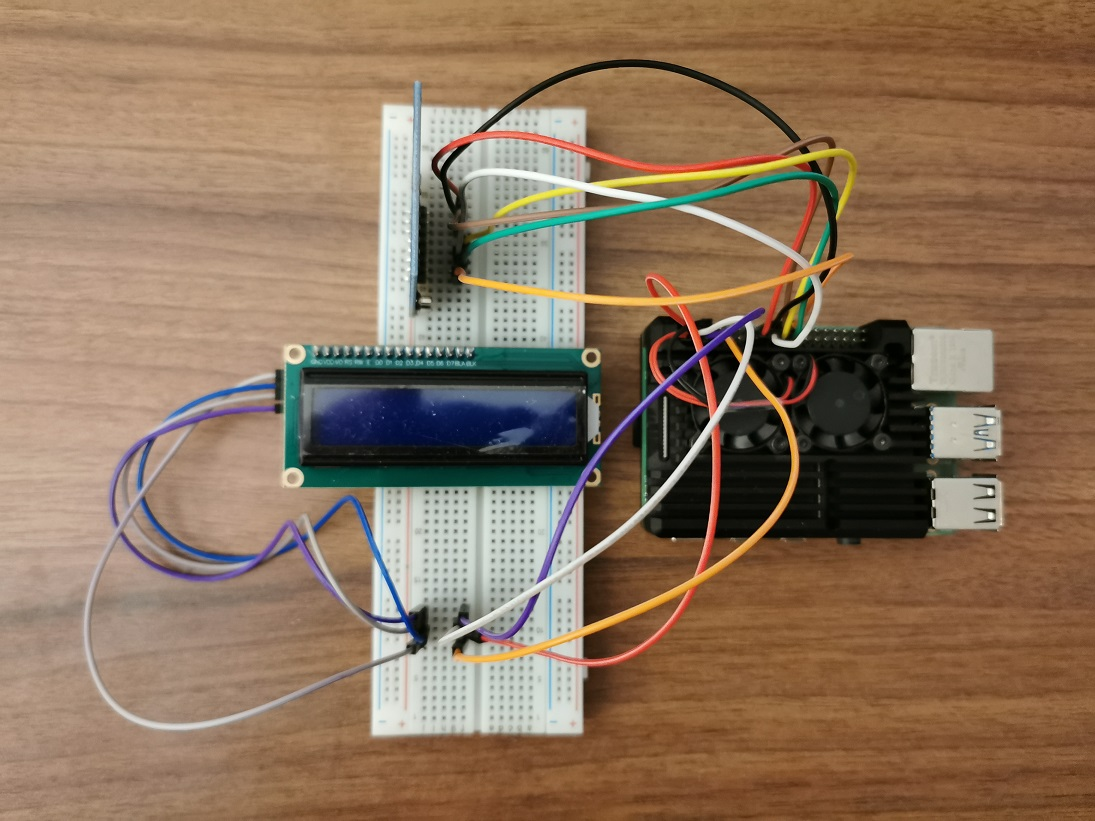
\includegraphics[width=0.7\linewidth]{img/1_kikapcsolt}
				\captionof{figure}{A rendszer kikapcsolt állapotban}
				\label{fig:1kikapcsolt}
			\end{minipage}
			\item Győződjön meg a kábelezés épségéről, szakadt kábel esetén a hibás vezetéket cserélni kell.
			\item Helyezze be az \textbf{USB-C} csatlakozót a \textbf{Raspberry Pi} egységbe.
			\item A rendszer indítása közben győződjön meg róla, hogy az \textbf{RFID olvasó} és az \textbf{LCD kijező} beépített LED-jei világítanak. \\
			\begin{minipage}{\linewidth}
				\centering
				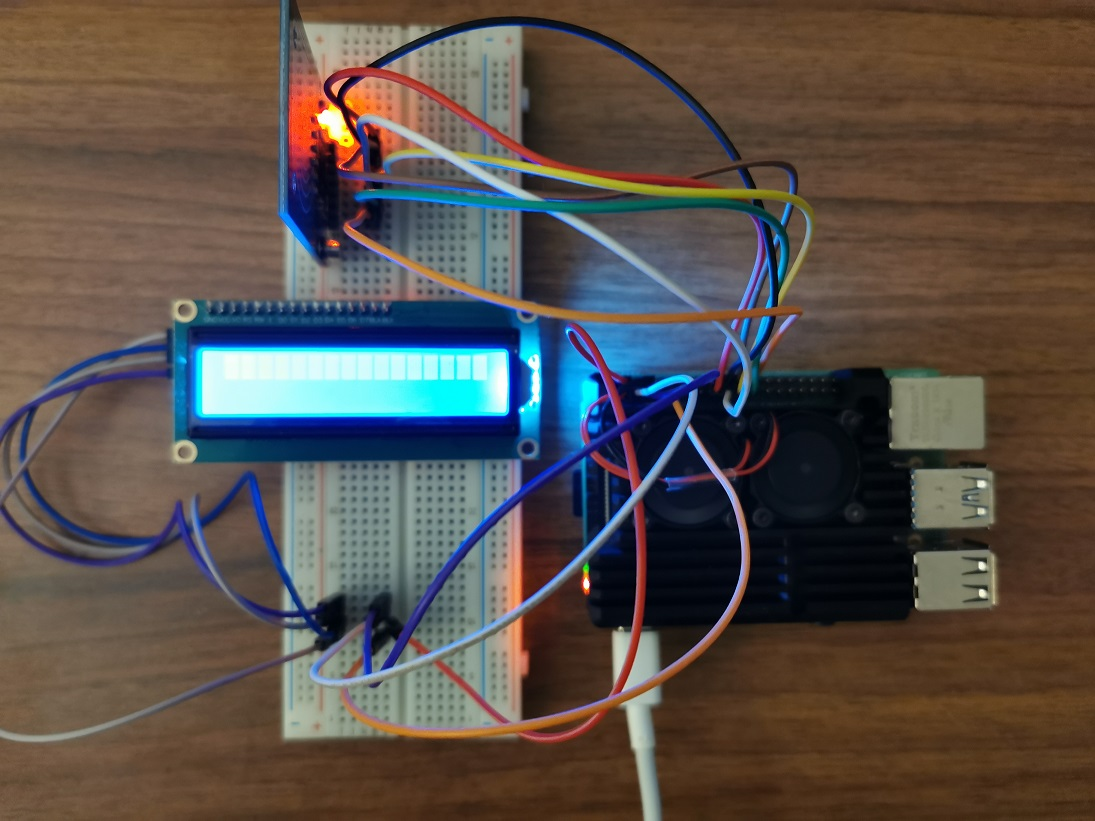
\includegraphics[width=0.7\linewidth]{img/2_indul}
				\captionof{figure}{A rendszer indítása}
				\label{fig:2indul}
			\end{minipage}
			\item Pár másodperc elteltével az \textbf{LCD kijelző}n meg kell jelennie a \emph{Kerem erintse a kartyajat!} szövegnek. \\
			\begin{minipage}{\linewidth}
				\centering
				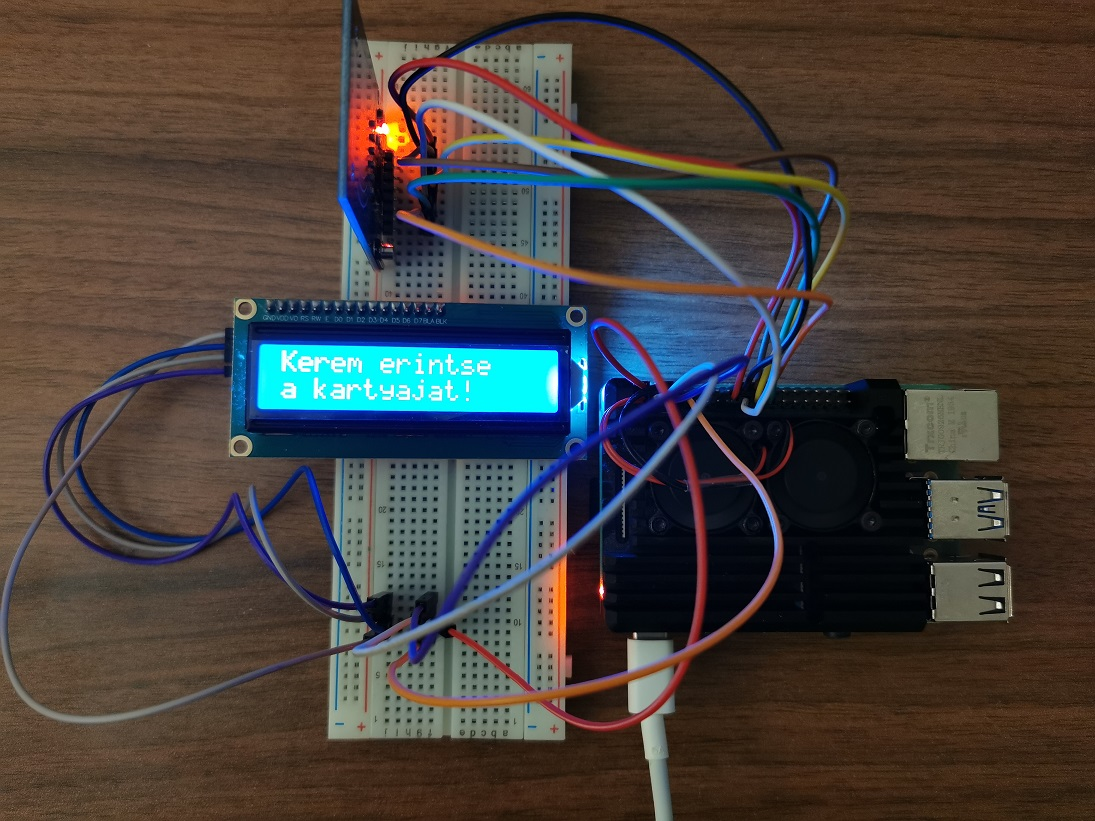
\includegraphics[width=0.7\linewidth]{img/3_futas}
				\captionof{figure}{A rendszer üzemkész állapotban}
				\label{fig:3futas}
			\end{minipage}
			\item A berendezés innentől kezdve rendeltetésszerűen használható. \\
		\end{enumerate}
		
	\section{Belépés RFID kulcs segítségével}
		\subsection{Sikeres belépési kísérlet}
			\begin{enumerate}
				\justifying
				\item Helyezze a kártyát vagy kulcsot a leolvasóhoz!
				\item Sikeres belépés esetén az \textbf{LCD kijelző}n megjelenik a \emph{Belepes engedelyezve!} szöveg \\
				\begin{minipage}{\linewidth}
					\centering
					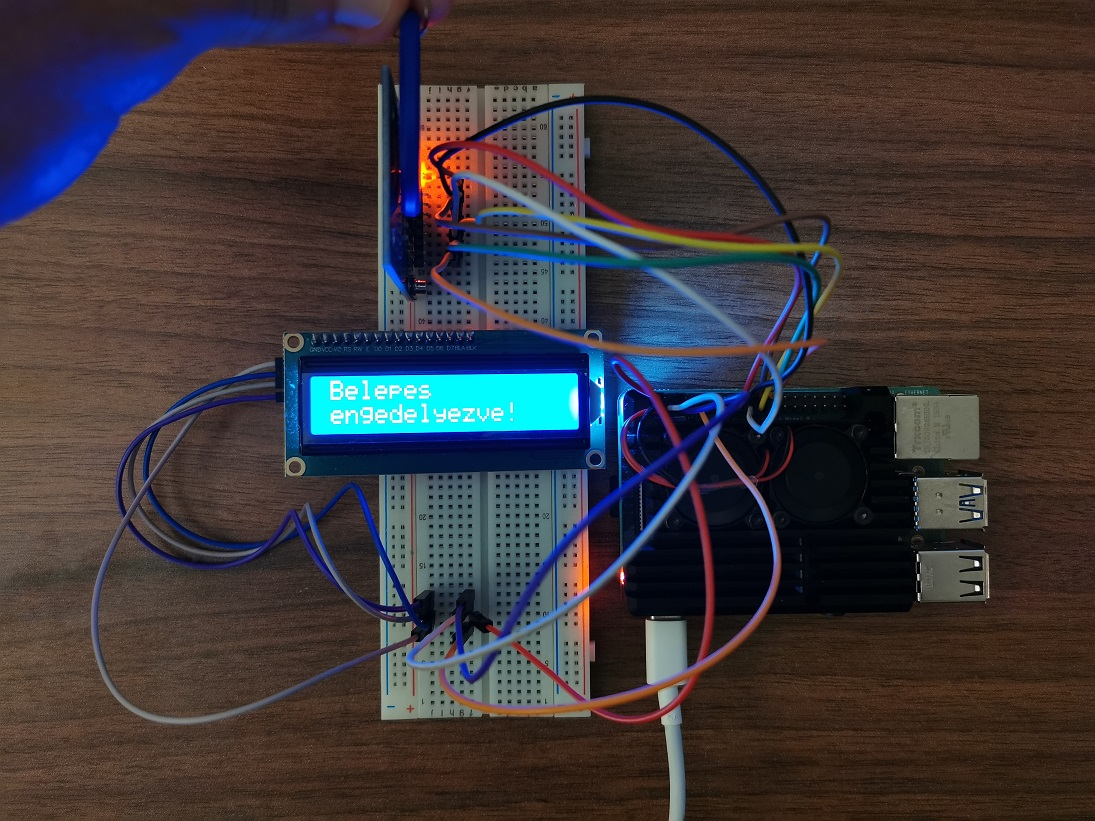
\includegraphics[width=0.7\linewidth]{img/4_engedelyezett}
					\captionof{figure}{Engedélyezett belépés}
					\label{fig:4engedelyezett}
				\end{minipage}
				\end{enumerate}
				\vfill
			\subsection{Belépési kísérlet tiltott kulccsal}
				\begin{enumerate}
					\justifying
					\item Helyezze a kártyát vagy kulcsot a leolvasóhoz!
					\item Ha kártyája vagy kulcsa le van tiltva, akkor belépés esetén az \textbf{LCD kijelző}n megjelenik a \emph{Kartya letiltva!} szöveg \\
					\begin{minipage}{\linewidth}
						\centering
						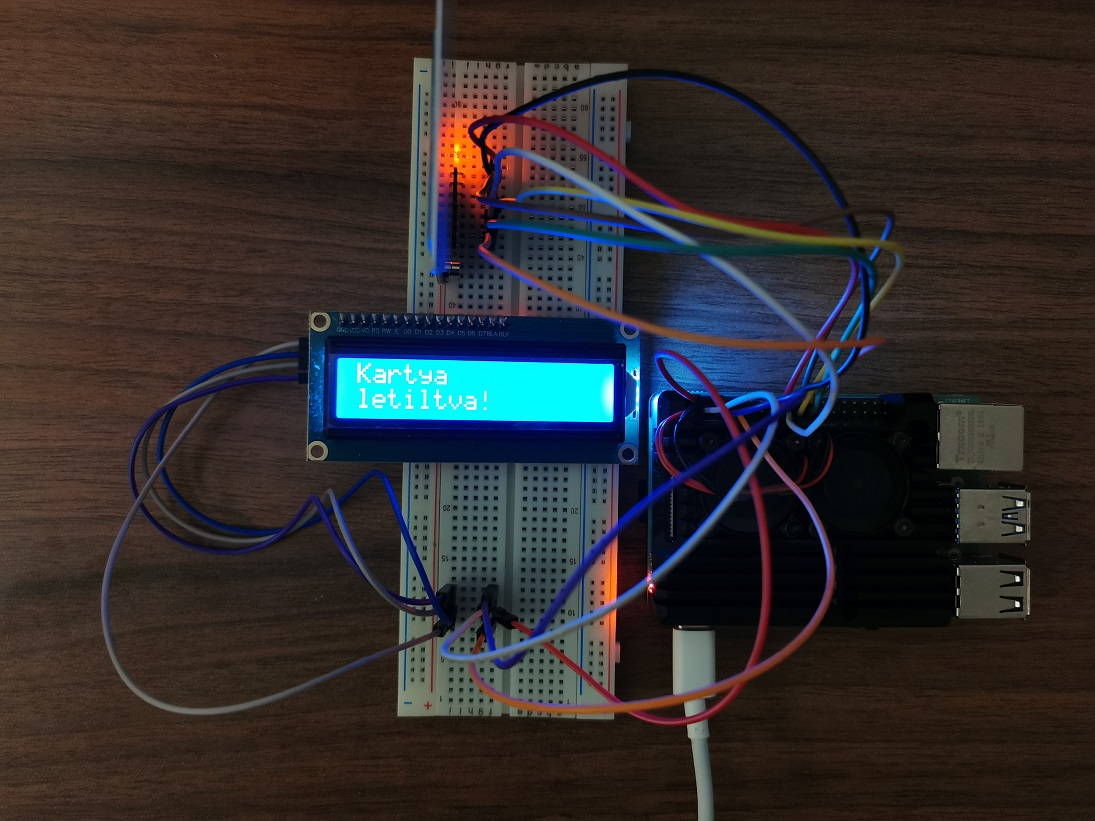
\includegraphics[width=0.7\linewidth]{img/5_letiltott}
						\captionof{figure}{Tiltott belépés}
						\label{fig:5letiltott}
					\end{minipage}
				\end{enumerate}
				\begin{flushleft}
					{\large\textbf{Figyelem!}} A rendszer többszöri letiltott kártya azonosítása esetén e-mailben fogja értesíteni a rendszergazdát az illetéktelen használatról!\\
					\begin{minipage}{\linewidth}
						\centering
						\begin{framed}
							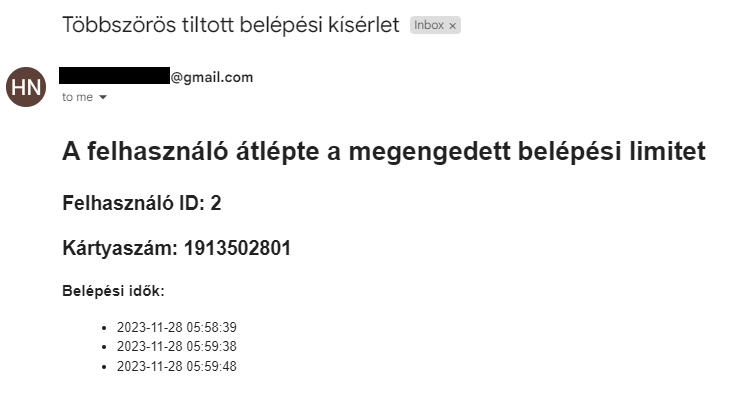
\includegraphics[width=1.0\linewidth]{img/6_limit_atlepes}
						\end{framed}
						\captionof{figure}{A megengedett limit átlépése}
						\label{fig:6limitatlepes}
					\end{minipage}
				\end{flushleft}
				\vfill
			\subsection{Belépési kísérlet ismeretlen kulccsal}
				\begin{enumerate}
					\justifying
					\item Helyezze a kártyát vagy kulcsot a leolvasóhoz!
					\item Ismeretlen azonosító esetén az \textbf{LCD kijelző}n megjelenik a \emph{Kartya nem ismert!} szöveg \\
					\begin{minipage}{\linewidth}
						\centering
						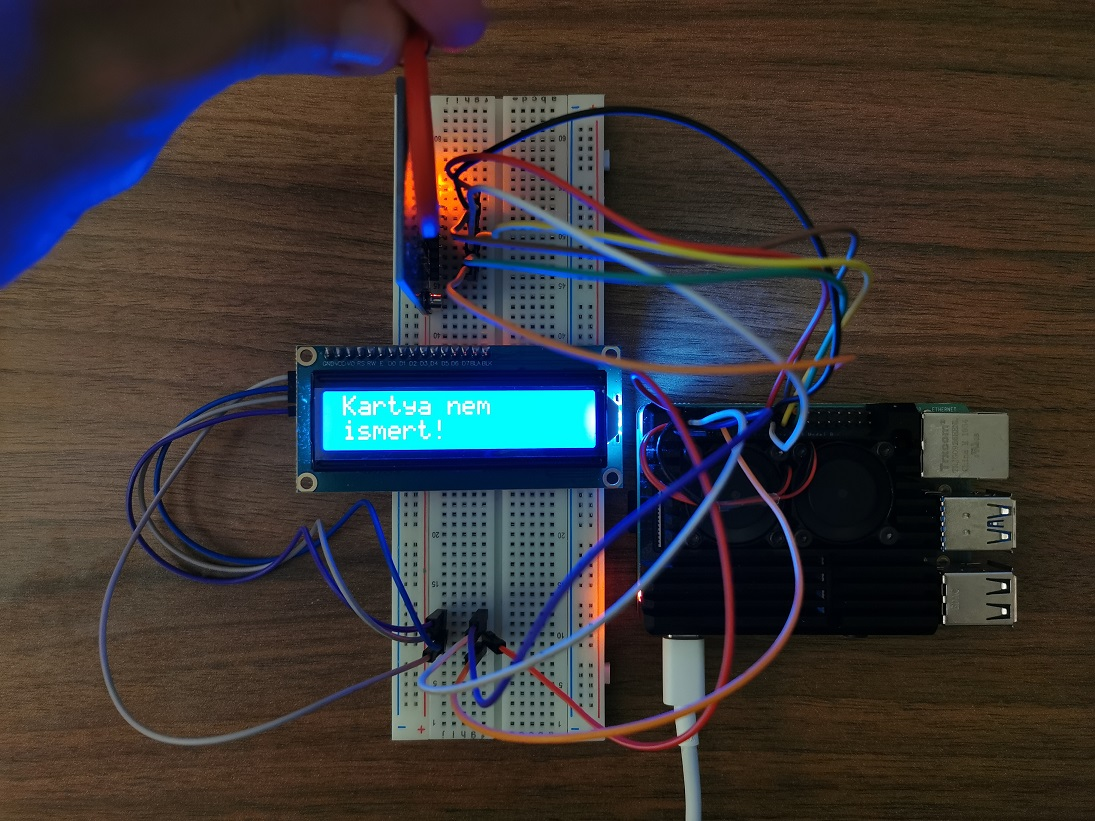
\includegraphics[width=0.7\linewidth]{img/7_nem_ismert}
						\captionof{figure}{Nem ismert azonosító}
						\label{fig:7nemismert}
					\end{minipage}
				\end{enumerate}
				\vfill
Ez a dokumentum a \color{blue} \href{https://www.latex-project.org/}{LaTeX} \color{black} szövegformázó rendszer segítségével jött létre.
\end{document}